\documentclass[10pt,a4paper]{article}
\usepackage[utf8]{inputenc}
\usepackage[italian]{babel}
\usepackage{amsmath}
\usepackage{amsfonts}
\usepackage{amssymb}
\usepackage{graphicx}
\usepackage[left=2cm,right=2cm,top=2cm,bottom=2cm]{geometry}
\newcommand{\rem}[1]{[\emph{#1}]}
\newcommand{\exn}{\phantom{xxx}}
\renewcommand{\thesubsection}{\thesection.\alph{subsection}}  %% use 1.a numbering

\author{Gruppo xxy \\ Luca Palumbo, Alessandro Costanzo Ciano \rem{non dimenticate di inserire i vostri nomi...}}
\title{Es04B: Circuiti lineari con Amplificatori Operazionali}
\begin{document}
\date{23 ottembre 2150 \rem{... ed anche la data corretta}}
\maketitle


\section*{Scopo dell'~esperienza}
Misurare le caratteristiche di circuiti lineari realizzati con un op-amp TL081 alimentato tra +5 V e -5 V.

\section*{A.Amplificatore non invertente}
Abbiamo realizzato un amplificatore non invertente con resistenza $R_1= 1 \rm \ k\Omega$  (nominale)
e con un'~amplificazione a centro-banda compresa tra 4 e 10 secondo lo schema mostrato in figura \ref{fig:noninv}.
%
\begin{figure}[h]
\begin{center}
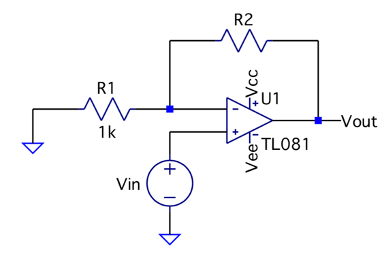
\includegraphics[width=0.4\linewidth]{ampl-noninv.png}
%\framebox(200,200){Inserire schema circuitale}
\caption{\small Schema dell'amplificatore non invertente}
\label{fig:noninv}
\end{center}
\end{figure}
%

%%%%%%%%%%%%%%%%%%%%%%%%%%%%%%%%%%%%%%%%%%%%%%%%%%%%%%
\section{Guadagno in tensione}
\subsection*{a.Misura delle resistenze}
Le resistenze selezionate hanno i seguenti valori, misurati con il multimetro digitale, con il corrispondente valore atteso 
del guadagno in tensione dell'~amplificatore.
\[
\begin{array}{l l l r}
    R_1 = ( 0.982 \pm 0.009) \,\mathrm{k}\Omega, & R_2 = (1.96 \pm 0.01) \,\mathrm{k}\Omega & \Rightarrow A_{v,exp} = ( 2.99 \pm 0.02) & \mbox{(Luca Palumbo)}\\
    R_1 = ( 5.08 \pm 0.06) \,\mathrm{k}\Omega, & R_2 = (0.991 \pm 0.003) \,\mathrm{k}\Omega & \Rightarrow A_{v,exp} = ( 1.195 \pm 0.002) & \mbox{(Alessandro C. Ciano)}
\end{array}
\]
\subsection*{b.Misura preliminare del guadagno}
Abbiamo inviato all'~ingresso dell'~amplificatore un segnale sinusoidale di frequenza $f_{in} = (1.00 \pm 0.01)$ kHz ed 
ampiezza $200\ \rm mV$. Ingresso ed uscita dell'~amplificatore sono mostrati in Fig. \ref{fig:oscnoninv}. Per le misure di ampiezza delle tensioni si è utilizzata la funzione "measurements" di Waveforms; l'errore associato è dato dalla somma della prima cifra instabile nella lettura, dai limiti di risoluzione dell'ADC e dallo 0.3\% del fondo scala. Otteniamo
\[
\begin{array}{llr}
V_{in} = (196  \pm 1) \ \rm mV,& V_{out} = (0.591 \pm 0.001) \ \rm V \Rightarrow A_v = ( 3.01 \pm 0.01) & \mbox{(ALuca Palumbo)}\\
V_{in} = (404 \pm 2) \ \rm mV, & V_{out} = ( 482 \pm 2) \ \rm mV \Rightarrow A_v = ( 1.193 \pm 0.006 ) & \mbox{(Alessandro C. Ciano)}
\end{array}
\]
%
\begin{figure}[h]
\begin{center}
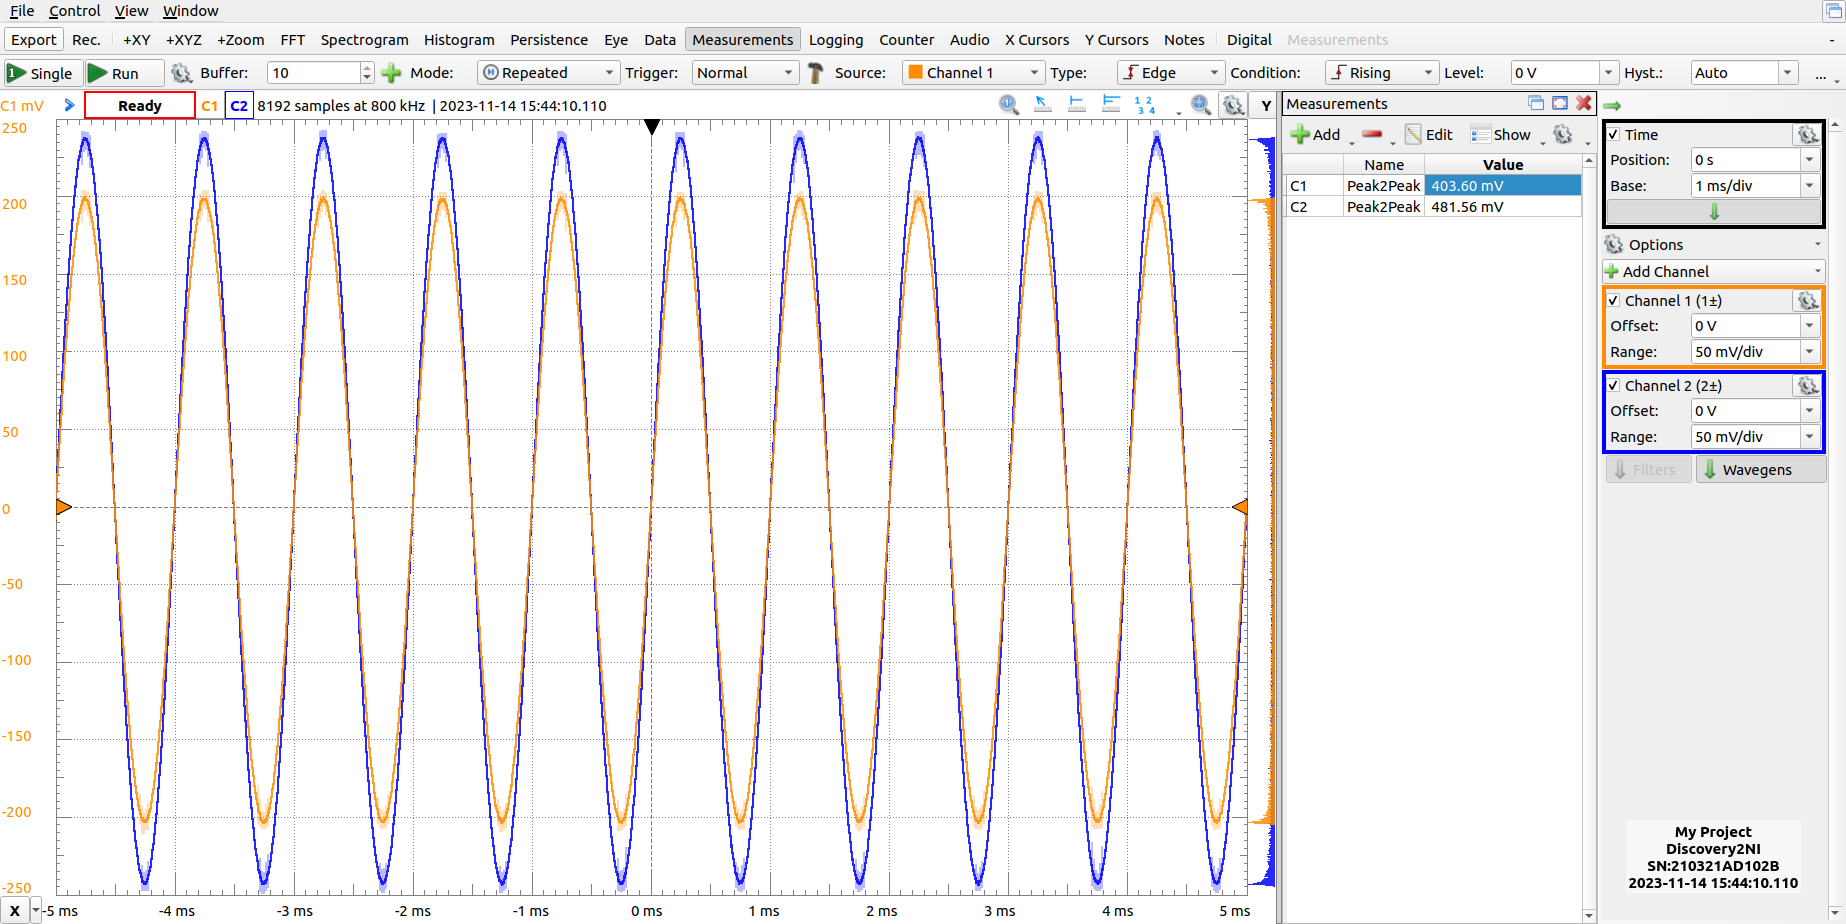
\includegraphics[width=0.75\textwidth]{oscilloscopio1.png}
\end{center}
\caption{\small Ingresso (primo canale) ed uscita (secondo canale) di un amplificatore non 
invertente con OpAmp per ampiezza di $V_{in}=200\ \rm mV$, riferito al ciruito di Alessandro C. Ciano}
\label{fig:oscnoninv}
\end{figure}
%

\subsection*{c.Verifica della linearit\`a e misura del guadagno}
Variando l'~ampiezza di $V_{in}$ abbiamo misurato $V_{out}$ e per ciascun valore ottenuto i guadagni $A_v=V_{out}/V_{in}
$ riportati in tabella~\ref{tab:guadagno}.
%
\begin{table}[h]
\caption{Ampiezza di $V_{out}$ in funzione di $V_{in}$ e relativo rapporto.}
\label{tab:guadagno}
\begin{center}
\begin{tabular}{|c|c|c|}
\hline
$V_{in}$ (mV) & $V_{out}$ (V)  & $A_v$ \\
\hline
\hline
$96 \pm 1 $ & $0.292 \pm 0.001 $ & $3.04 \pm 0.03$ \\
\hline
$196 \pm 1 $ & $0.592 \pm 0.002 $ & $3.02 \pm 0.02 $ \\
\hline
$296 \pm 1 $ & $0.892 \pm 0.002 $ & $3.01 \pm 0.01 $ \\
\hline
$397 \pm 1 $ & $1.192 \pm 0.002 $ & $3.00 \pm 0.01 $ \\
\hline
$496 \pm 1 $ & $1.492 \pm 0.002 $ & $3.00 \pm 0.01 $ \\
\hline
\end{tabular}
\end{center}
\end{table}

Si è considerato come intervallo di linearità l'intero set di misue, in quento tutti i guadagni risultano tra loro compatibili.
Utilizzando i soli dati in questo intervallo abbiamo effettuato un'~interpolazione di ($V_{out}$ oppure $A_v$, \rem{scegliere 
quale}) in funzione di $V_{in}$ ($V_{out}=AV_{in}$). Il risultato del fit \`e riportato nel grafico di Fig. \ref{fig:lin}, 
con sovrapposta la funzione di best-fit, insieme all'~andamento degli scarti normalizzati. Determiniamo cos\`\i\  la nostra migliore 
stima del guadagno mediante fit dei dati ottenuti:
\[
A_{best} = 3.010 \pm 0.002 \quad,\quad  \chi^2/\mbox{n.d.o.f.} = 13/4.
\]
Il valore del guadagno ottenuto dal best fit risulta in accordo con quello atteso dalle misure delle resistenze. Il $\chi^2$ risulta ragionevole date le poche misure a disposizione.
\begin{figure}[t]
\begin{center}
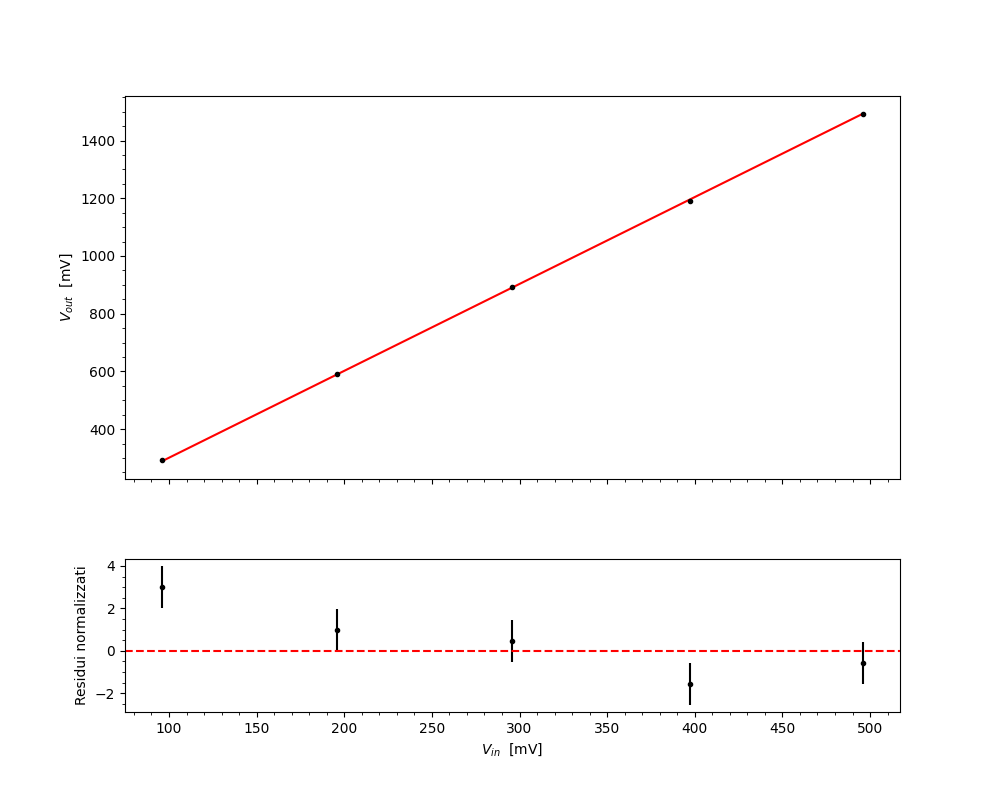
\includegraphics[width=0.8\textwidth]{fitconresidui4.png}
\end{center}
\caption{\small Andamenti in funzione di $V_{in}$ di: (sopra) $V_{out}$, con verifica della inearit\`a dell'~amplificatore, e (sotto) 
dei scarti normalizzati rispetto alla funzione di best-fit.}
\label{fig:lin}
\end{figure}
%
%%%%%%%%%%%%%%%%%%
%
\section{Risposta in frequenza del circuito}
Abbiamo misurato la risposta in frequenza dell'~amplificatore utilizzando Network Analyzer ed ottenendo i plot di Bode mostrati 
in Fig. \ref{fig:bodenoninv}. Il guadagno di centro-banda risulta essere $A_M (dB) = (9.52 \pm 0.06 ) \ \rm dB$, o in unità naturali $A_M (dB) = (2.99 \pm  0.02)$, perfettamente in accordo con i risultati della regressione lineare precedente. La nostra migliore determinazione per 
la frequenza di taglio superiore \`e
\[
f_L = (0.852 \pm 0.005 ) \  \rm MHz
\]
determinata attraverso la riduzione del guadagno in tensione di 3dB rispetto a centro-banda. 

\begin{figure}[h]
\begin{center}
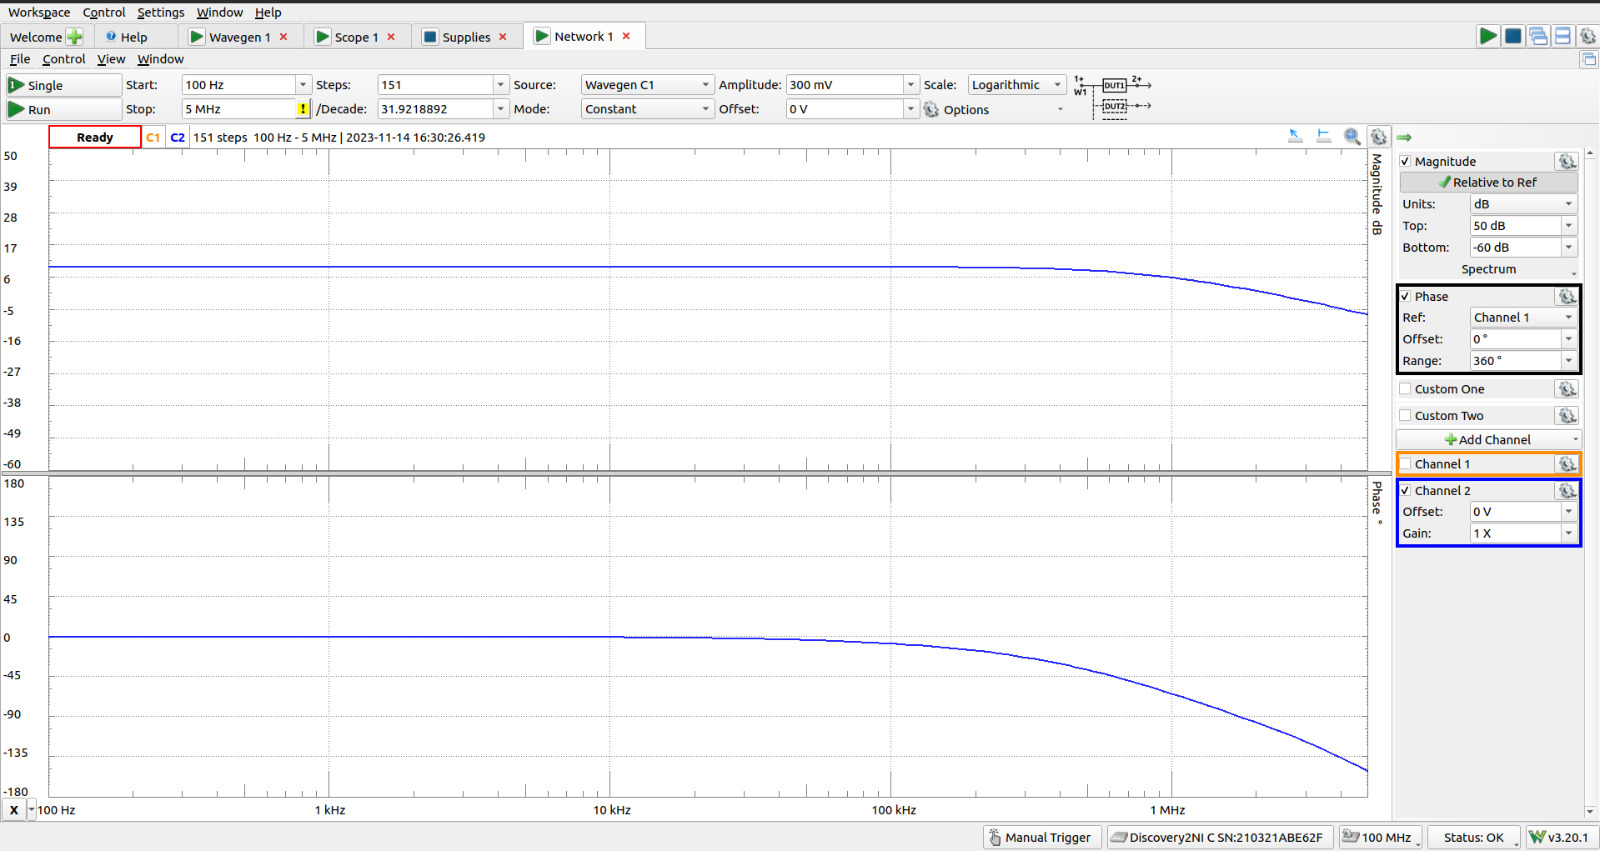
\includegraphics[width=0.7\textwidth]{bode.jpeg}
\caption{\small Plot di Bode in ampiezza (sopra) e fase (sotto) per l'~amplificatore non invertente.}
\label{fig:bodenoninv}
\end{center}
\end{figure}
%
Moltiplicando questa frequenza per il guadagno di centro-banda otteniamo la seguente stima del prodotto banda-guadagno
\[
\mbox{GBW} = A_M f_L = (2.57 \pm 0.02)\ \rm MHz
\]
da confrontarsi con un valore tipico di \exn riportato dal data sheet dell'opamp \rem{citare quello ottenuto dal costruttore nelle 
condizioni di test pi\`u vicine a quelle di misura}.
%
\section{Misura dello \emph{slew-rate}}
Si misura direttamente lo \emph{slew-rate} del TL081 dalla pendenza di $V_{out}$ in corrispondenza dei fronti di salita/discesa 
di un'~onda quadra di frequenza di $(1.00 \pm 0.01) \ \rm kHz$ ed ampiezza $(2.039 \pm 1) \ \rm V$ inviata all'~ingresso 
dell'~amplificatore. Uno screenshot dei due segnali \`e visibile in figura \ref{fig:slew}. Si ottiene:
\[
\mbox{SR} = (13.0 \pm 0.1 )\ \rm V/\mu s \quad \mathrm{valore \; tipico}\, 
\]
contro un valore tipico di $(13 ) \  \rm V/\mu s$ quotato dal data-sheet, in accordo col precedente.
%
\begin{figure}[h]
\begin{center}
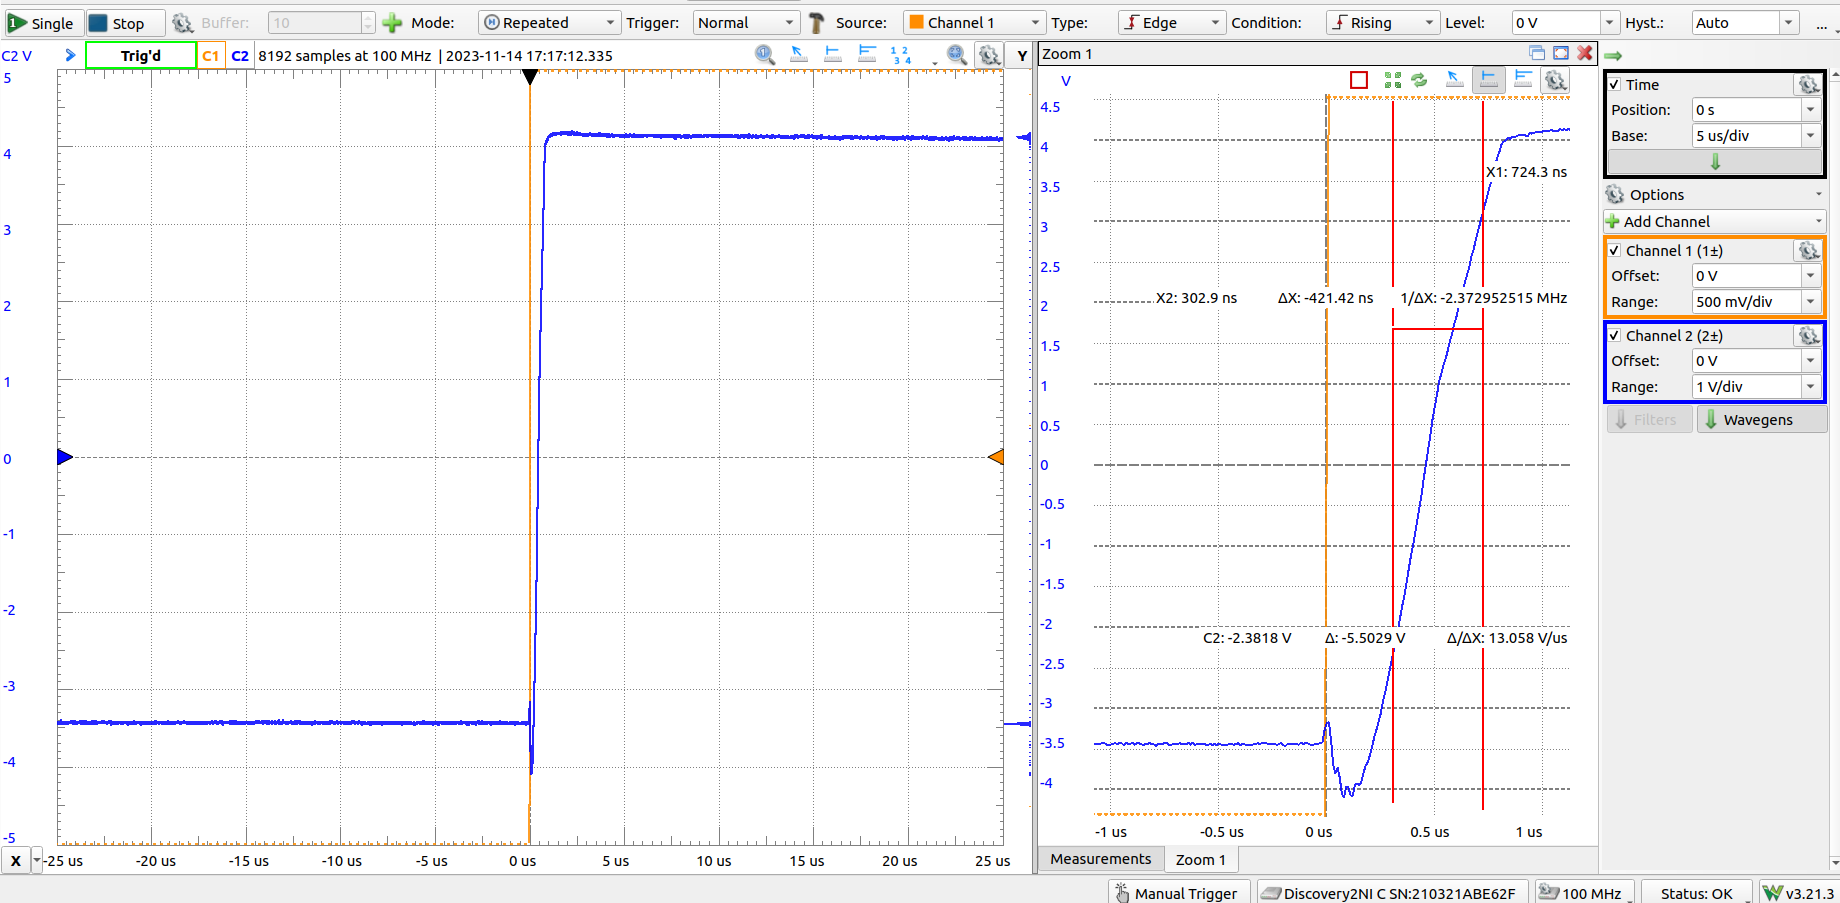
\includegraphics[width=0.7\textwidth]{slewrate.png}
\caption{\small Fronti dei segnali per la misura dello slew-rate del TL081.}
\label{fig:slew}
\end{center}
\end{figure}
%
\section{Circuito derivatore}
\subsection*{a.Montaggio del circuito}
Abbiamo realizzato un circuito derivatore reale con i seguenti valori dei componenti indicati: 
\[
\begin{array}{lll}
R_1 & = & (0.993 \pm 0.09) \  \rm k\Omega\\
R_2 & = & (9.96 \pm 0.009) \  \rm k\Omega\\ 
C_1 & = & (47.0 \pm 2.2) \  \rm nF
\end{array}
\]
%
\subsection*{b.Risposta in frequenza}
Di nuovo utilizzando Network Analyzer abbiamo ottenuto i plot di Bode mostrati
in Fig. \ref{fig:bodederiv}. 
L'~andamento a basse frequenze \`e quello tipico di un filtro passa-alto con frequenza di taglio 
\[
f_H = (3.37+ \pm 0.03 )  \  \rm kHz
\]
anche in questo caso determinata attraverso la riduzione del guadagno in tensione di 3dB rispetto a centro-banda. 
%
\begin{figure}[h]
\begin{center}
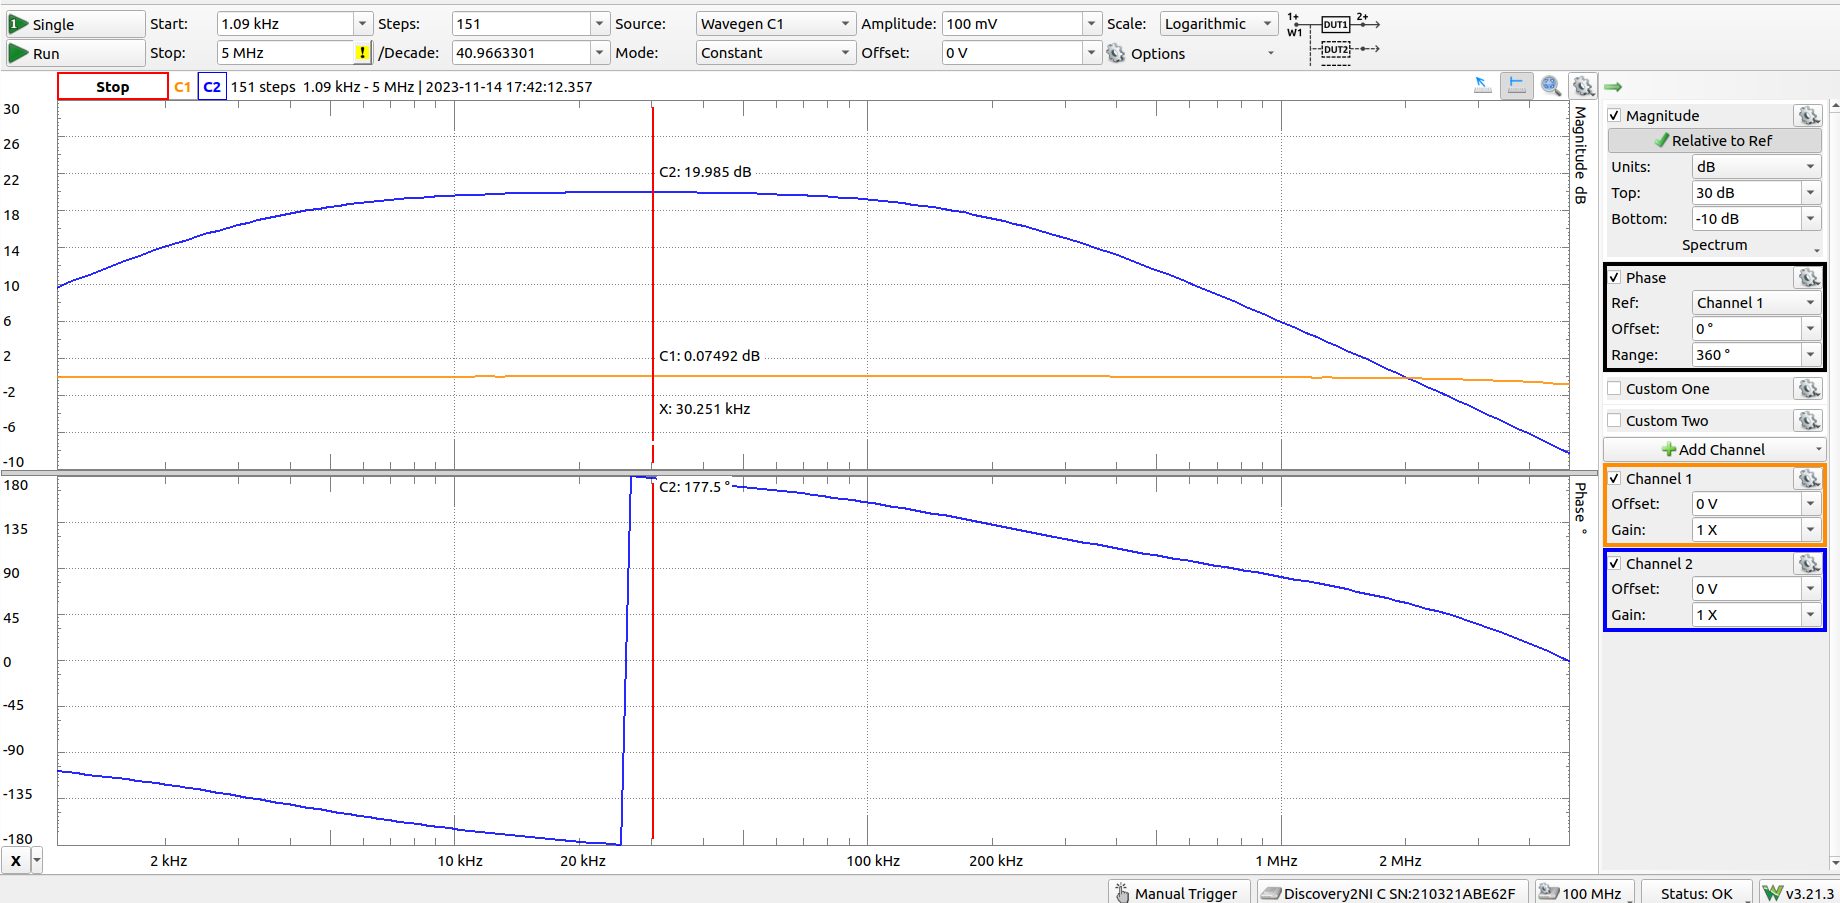
\includegraphics[width=0.7\textwidth]{bodeplot2.png}
\caption{\small Plot di Bode in ampiezza (sopra) e fase (sotto) per il circuito derivatore.}
\label{fig:bodederiv}
\end{center}
\end{figure}
%
\subsection*{c.Risposta ad un'~onda triangolare}
Abbiamo inviato all'~ingresso del circuito un'~onda triangolare simmetrica di frequenza $(100 \pm 1) \ \rm Hz$ ed ampiezza 
$(497 \pm 2) \ \rm mV$. Si riportano in Fig. \ref{fig:oscderiv} le forme d'~onda acquisite all'~oscillografo per l'~ingresso
e l'~uscita. $V_{out}$ risulta avere la formad di un'onda quadra, come atteso dal comportamento di un derivatore. Essendo il guadagno del circuito $A=-\dfrac{-R_2}{R_1}\dfrac{j\omega R_1 C}{1+j\omega R_1 C}$, nel limite di basse frequenze ($\omega << \dfrac{1}{R_1 C}$) si ha $A\approx -j\omega R_2 C$, tipica di un derivatore. 
L'~ampiezza di $V_{out}$ - misurata con i cursori il valore centrale del massimo assunto, avendo cura di considerare anche un'incertezza dovuta al rumore - \`e $V_M =  (368.56 \pm 12) \ \rm mV$. 
%
\begin{figure}[htb]
\begin{center}
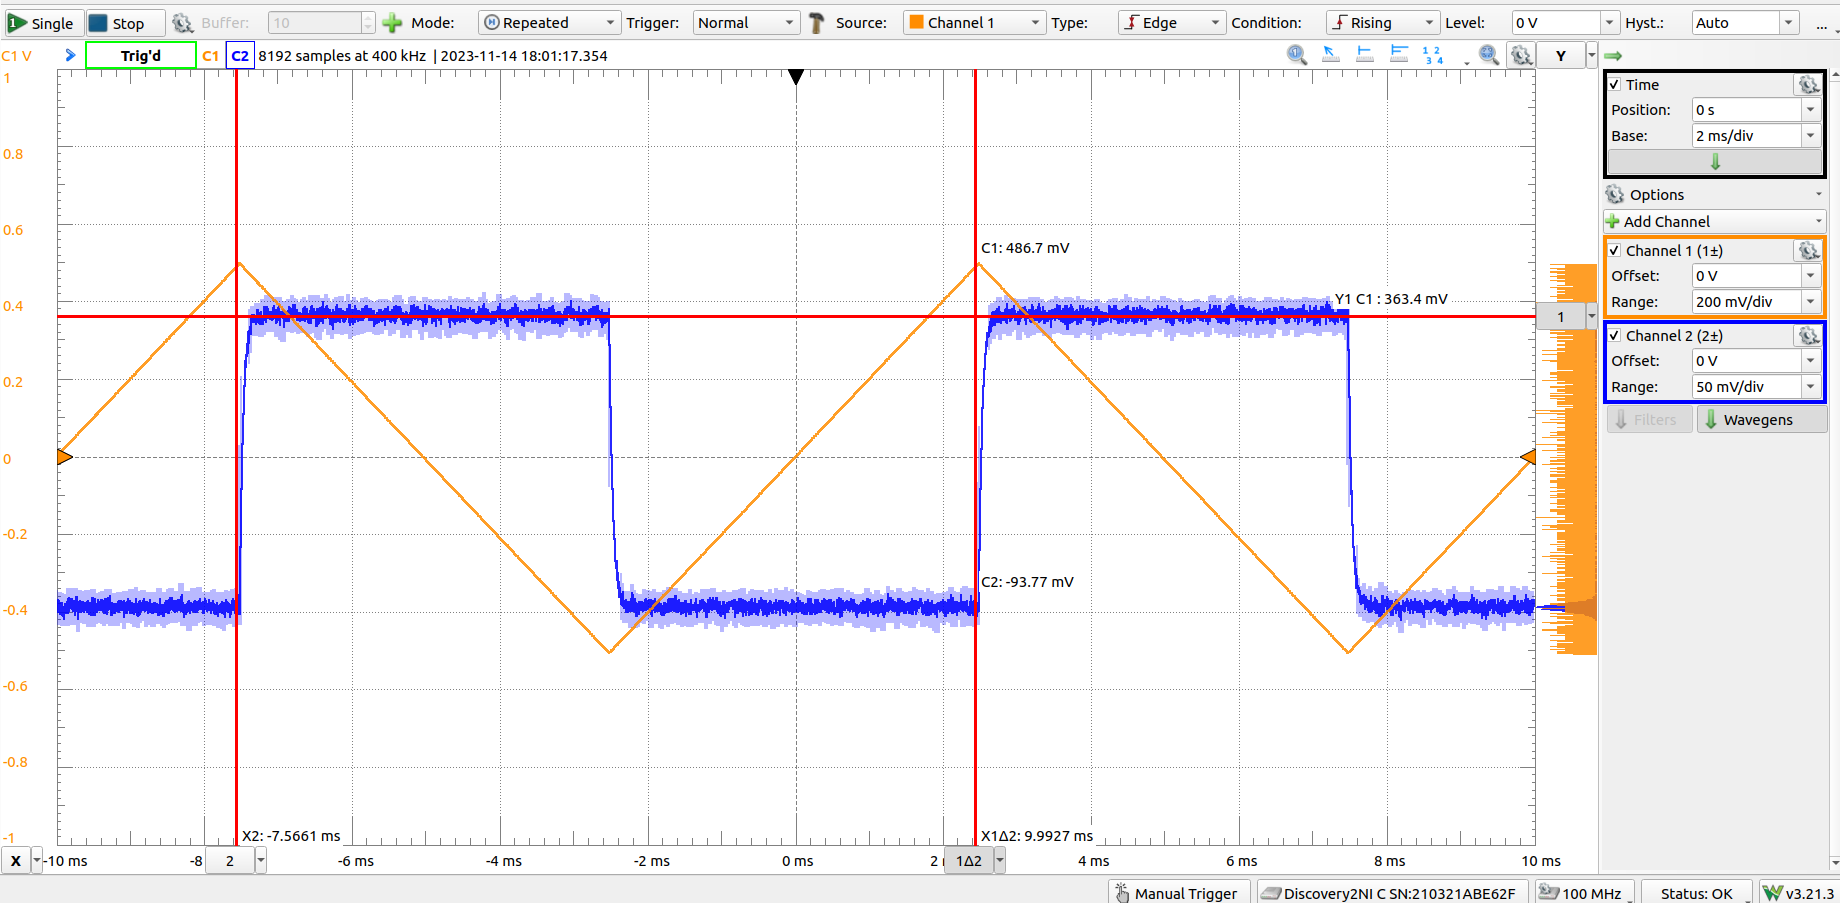
\includegraphics[width=0.75\textwidth]{derivatore.png}
\caption{\small Ingresso (Ch1) ed uscita (Ch2) del circuito derivatore in risposta ad un'~onda triangolare di frequenza 100 Hz.}
\label{fig:oscderiv}
\end{center}
\end{figure}
%
\subsection*{d.Confronto con i valori attesi}
Sulla base dei valori misurati dei componenti, il valore atteso per la frequenza di taglio del circuito \`e $f_{H,exp} = \dfrac{1}{2\pi R_1 C} = 
(3.4 \pm 0.2) \ \rm kHz$, in ottimo accordo con la misura. 

Per l'~ampiezza dell'~onda quadra in uscita a $100 \ \rm Hz$ ci aspettiamo perci\`o un valore di 
\[
V_M = \omega R_2 C V_{in}= ( \pm ) \ \rm mV
\]
\subsection*{e.Dipendenza della risposta dalla frequenza}
\rem{Inserire commenti su quanto osservato, eventualmente servendosi di appositi screenshot dell'oscillografo} 

%%%%%%%%%%%%%%%%%%%%%%%%

\end{document}          
